\documentclass[tikz]{standalone}
\begin{document}
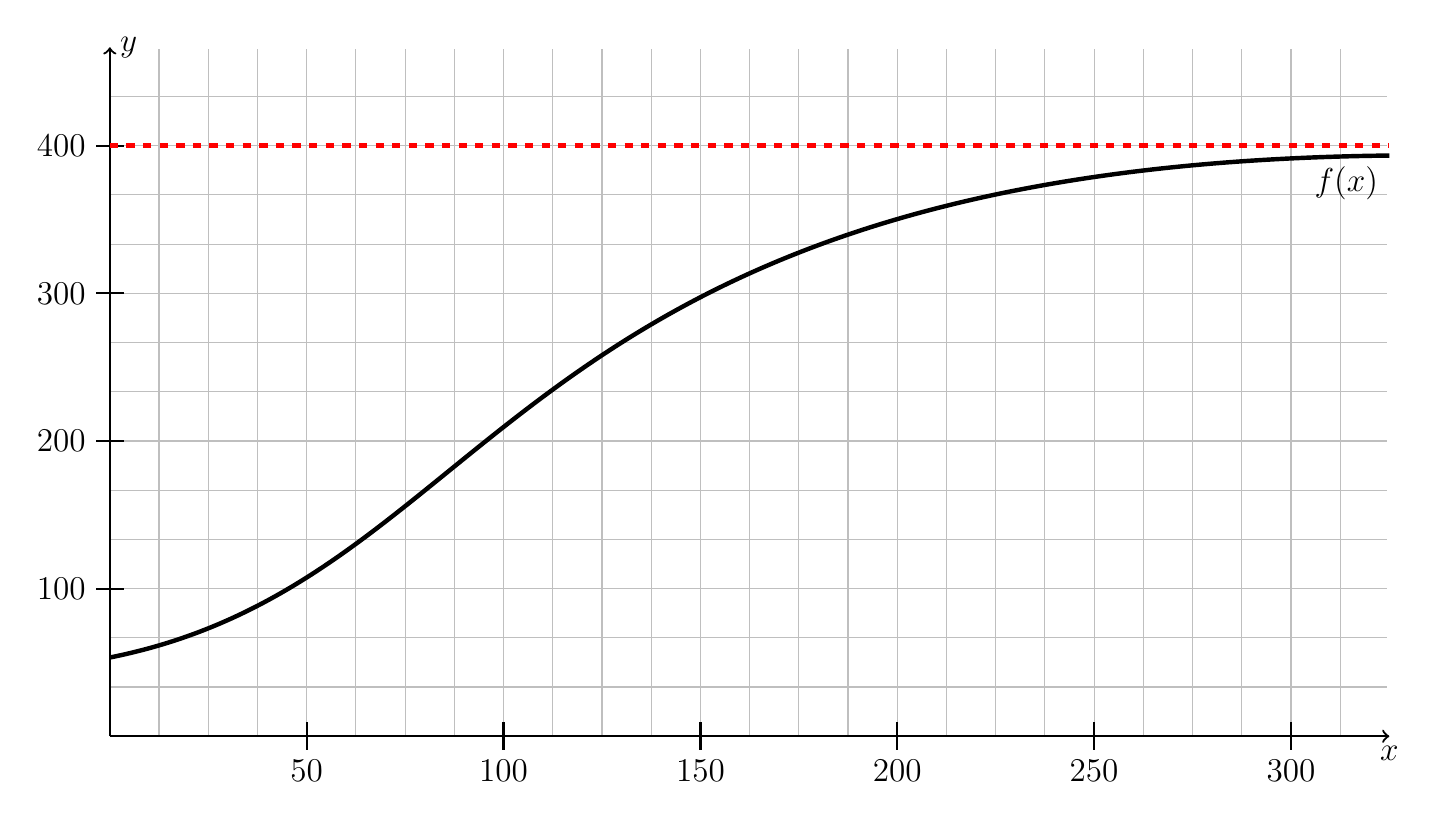
\begin{tikzpicture}[scale=2.5]
\tikzstyle{every node}=[font=\large]
 
% create a white background, with a black frame
%\draw [fill=white,white] (-0.75,-0.5) rectangle (6.75,3.75); 

% draw a grid
\draw[step=2.5mm, lightgray, thin] (0,0) grid (6.49,3.49); 

% draw axes
\draw [->,thick] (0,0) -- (6.5,0) node[below] {$x$}; 
\draw [->,thick] (0,0) -- (0,3.5) node[right] {$y$};

% tick marks
\foreach \x/\label in {1/50,2/100,3/150,4/200,5/250,6/300} 
	\draw [thick] (\x cm,2pt) -- (\x cm,-2pt) node[below] {\label};
\foreach \y/\label in {0.75/100,1.5/200,2.25/300,3/400} 
	\draw [thick] (2pt,\y cm) -- (-2pt,\y cm) node[left] {\label};

% plot curve
\draw [dashed, red,ultra thick](0,3) -- (6.5,3);
\draw [ultra thick] (0,0.4) .. controls (2,0.8) and (2,2.9) .. (6.5,2.95) node[below left] {\large $f(x)$};

\end{tikzpicture}
\end{document} 
